\documentclass[a4paper,12pt]{article}
\usepackage{amsmath}
\usepackage{amssymb}
\usepackage[polish]{babel}
\usepackage{polski}
\usepackage[utf8]{inputenc}
\usepackage{indentfirst}
\usepackage{geometry}
\usepackage{array}
\usepackage[pdftex]{color,graphicx}
\usepackage{subfigure}
\usepackage{afterpage}
\usepackage{setspace}
\usepackage{color}
\usepackage{wrapfig}
\usepackage{listings}
\usepackage{datetime}

\renewcommand{\onehalfspacing}{\setstretch{1.6}}

\geometry{tmargin=2.5cm,bmargin=2.5cm,lmargin=2.5cm,rmargin=2.5cm}
\setlength{\parindent}{1cm}
\setlength{\parskip}{0mm}

\newenvironment{lista}{
\begin{itemize}
  \setlength{\itemsep}{1pt}
  \setlength{\parskip}{0pt}
  \setlength{\parsep}{0pt}
}{\end{itemize}}

\newcommand{\linia}{\rule{\linewidth}{0.4mm}}

\definecolor{lbcolor}{rgb}{0.95,0.95,0.95}
\lstset{
    backgroundcolor=\color{lbcolor},
    tabsize=4,
  language=C++,
  captionpos=b,
  tabsize=3,
  frame=lines,
  numbers=left,
  numberstyle=\tiny,
  numbersep=5pt,
  breaklines=true,
  showstringspaces=false,
  basicstyle=\footnotesize,
  identifierstyle=\color{magenta},
  keywordstyle=\color[rgb]{0,0,1},
  commentstyle=\color{Darkgreen},
  stringstyle=\color{red}
  }

\begin{document}

\noindent
\begin{tabular}{|c|p{11cm}|c|} \hline 
Grupa 3 & Albert Soczewski, Maciej Ząbek & \ddmmyyyydate\today \tabularnewline
\hline 
\end{tabular}


\section*{Zadanie 1 - Rozmycie Gaussa w OpenMP}

Celem zadania było wykonanie programu rozmywającego zadane zdjęcie za pomocą algorytmu Gaussa z maską o wymiarach 5x5. Do zrównoleglenia operacji wykorzystana została biblioteka OpenMP, natomiast funkcjonalości potrzebne do pracy z obrazami zapewnione zostały dzięki bibliotece OpenCV.\\W programie została wykorzystana przedstawiona poniżej maska:

\begin{figure}[ht]
\centering
\begin{tabular}{|l|l|l|l|l|}
\hline
0 & 1 & 2 & 1 & 0 \\ \hline
1 & 4 & 8 & 4 & 1 \\ \hline
2 & 8 & 16 & 8 & 2 \\ \hline
1 & 4 & 8 & 4 & 1 \\ \hline
0 & 1 & 2 & 1 & 0 \\ \hline
\end{tabular}
\caption{Zastosowany filtr wykorzystujący funkcje Gaussa}
\end{figure}

\noindent Poniżej zaprezentowano algorytm rozmycia. Zmiennymi wspólnymi dla wątków są obrazy (wejściowy oraz wyjściowy) oraz liczba wątków. 

\begin{lstlisting}
#pragma omp parallel for shared(inputImage, outputImage, weight) num_threads(threads) private(red,green,blue,y,x) schedule(static)
 	for (y = 2; y < inputImage.rows - 2; y++) {
        for (x = 2; x < inputImage.cols - 2; x++) {
            red = 0; green = 0; blue = 0;
            for (int y_m = 0; y_m<5; y_m++) {
                for (int x_m = 0; x_m<5; x_m++) {
                    Vec3b intensity = inputImage.at <Vec3b>(y_m + y - 2, x_m + x - 2);

                    red += intensity.val[2] * mask[x_m][y_m];
                    green += intensity.val[1] * mask[x_m][y_m];
                    blue += intensity.val[0] * mask[x_m][y_m];
                }
            }
            Vec3b masks = Vec3b();
            masks.val[2] = red / weight;
            masks.val[1] = green / weight;
            masks.val[0] = blue / weight;
            outputImage.at<Vec3b>(y - 2, x - 2) = masks;
        }
    }
\end{lstlisting}

Algorytm dla każdego piksela (z pominięciem ramki) pobiera wartości kolorów składowych, wyznacza nową wartość piksela (na podstawie otaczających go sąsiadów) oraz dokonuje zapisu na nowym obrazie. \newline

\noindent W celu uzyskania odpowiednich rezultatów, do wczytanego obrazu dodana zostaje ramka złożona z kopii pikseli brzegowych. 

\begin{lstlisting}
 copyMakeBorder(inputImage, inputImage, 2, 2, 2, 2, BORDER_REPLICATE);
\end{lstlisting}

\newpage

\noindent Poniższy wykres przedstawia zależność czasu wykonywania programu od liczby wykorzysywanych wątków. Badany obraz miał wymiary 4032x2268px.

\begin{figure}[!ht]
	\centering
 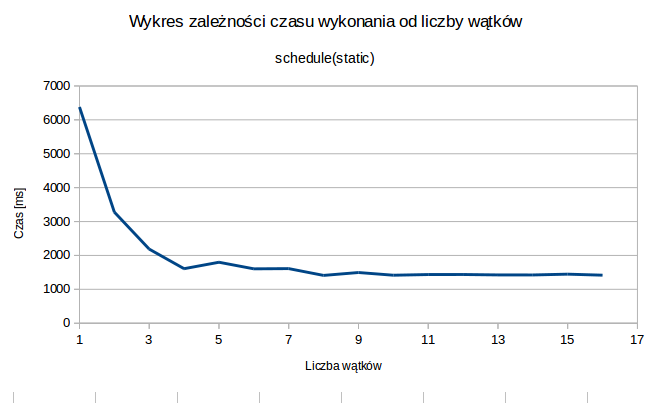
\includegraphics[width=0.7\textwidth]{./dane/wykres1_s.png}
  \caption{Wykres zależności czasu wykonania od liczby wątków}
\end{figure}

Na wykresie można zaobserwować, że w czas wykonania malał gdy liczba wątków się zwiększała. Najwiekszą poprawę zanotowano dla pierwszych 4 wątków. Nieco wolniej malał aż do wykorzystania 8 wątków, po osiągnięciu których ustabilizował się. Wynika to z faktu, że największy zysk przyspieszenia uzyskujemy uruchamiając pierwsze dodatkowe wątki. Korzystając z wielu wątków procesora, zysk nie jest już tak imponujący. Potwierdza to wykres przyspieszenia umieszczony poniżej.

\begin{figure}[ht]
	\centering
  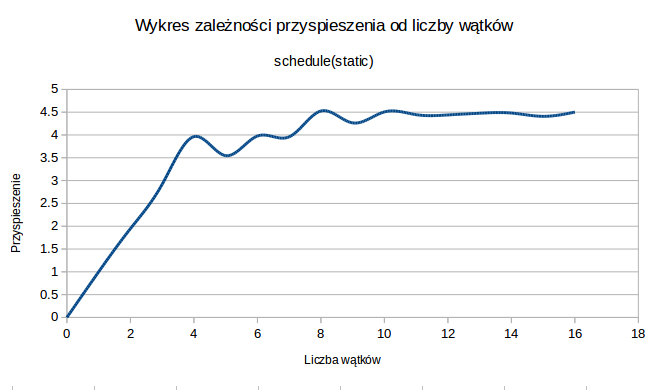
\includegraphics[width=0.7\textwidth]{./dane/wykres2_s.png}
  \caption{Wykres zależności przyspieszenia od liczby wątków}
\end{figure}

Zrównoleglając operacje udało się uzyskać niemalże 4,5 krotne przyspieszenie, co jest satysfakcjonującym wynikiem. Warto zauważyć także nieoczekiwany wzrost czasu wykonania dla wykonywania operacji na 5,6 oraz 7 wątkach. Wynika to z faktu, że do dyspozycji mamy 4 rdzenie procesora - 4 wątki. Przy użyciu dyrektywy schedule z argumentem static w wspomnianych wyżej przypadkach wątki oczekują na możliwość przeprowadzenia operacji. Problem ten rozwiązuje użycie dyrektywy dynamic, dzięki której wątki otrzymują kolejną porcje iteracji do wykonania od razu po zakończeniu obliczen. Tę sytuację przedstawia wykres poniżej.

\begin{figure}[ht]
	\centering
  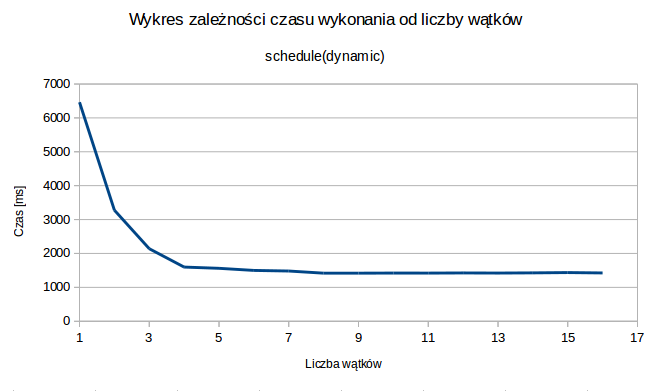
\includegraphics[width=0.7\textwidth]{./dane/wykres1_d.png}
  \caption{Wykres zależności przyspieszenia od liczby wątków}
\end{figure}

\end{document}